\documentclass[tikz,border=5pt]{standalone}
\usepackage[T1]{fontenc}
\usetikzlibrary{arrows.meta,positioning}
\definecolor{sourcecolor}{HTML}{B45332}
\definecolor{revisioncolor}{HTML}{246D92}
\definecolor{baselinecolor}{HTML}{8B6B9F}
\definecolor{inkcolor}{HTML}{253444}
\definecolor{gatecolor}{HTML}{EAF2F7}
\begin{document}
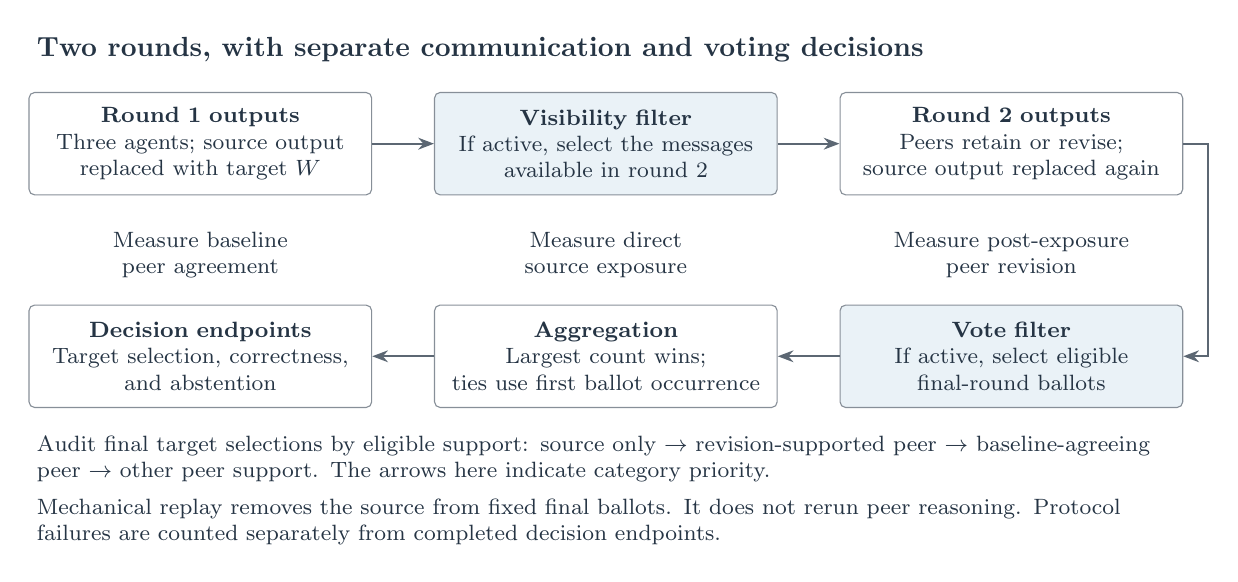
\begin{tikzpicture}[x=1cm,y=1cm,font=\footnotesize,text=inkcolor,
 stage/.style={draw=inkcolor!55,rounded corners=2pt,align=center,text width=4cm,minimum height=1.3cm,inner sep=5pt},
 flow/.style={-{Stealth[length=2mm]},thick,draw=inkcolor!75}]
\node[anchor=west,font=\bfseries] at (0,0.5) {Two rounds, with separate communication and voting decisions};
\node[stage] (roundone) at (2.2,-0.7) {\textbf{Round 1 outputs}\\Three agents; source output\\replaced with target $W$};
\node[stage,fill=gatecolor] (visibility) at (7.35,-0.7) {\textbf{Visibility filter}\\If active, select the messages\\available in round 2};
\node[stage] (roundtwo) at (12.5,-0.7) {\textbf{Round 2 outputs}\\Peers retain or revise;\\source output replaced again};
\node[stage,fill=gatecolor] (voting) at (12.5,-3.4) {\textbf{Vote filter}\\If active, select eligible\\final-round ballots};
\node[stage] (aggregate) at (7.35,-3.4) {\textbf{Aggregation}\\Largest count wins;\\ties use first ballot occurrence};
\node[stage] (outcome) at (2.2,-3.4) {\textbf{Decision endpoints}\\Target selection, correctness,\\and abstention};
\draw[flow] (roundone) -- (visibility);
\draw[flow] (visibility) -- (roundtwo);
\draw[flow] (roundtwo.east) -- (15,-0.7) -- (15,-3.4) -- (voting.east);
\draw[flow] (voting) -- (aggregate);
\draw[flow] (aggregate) -- (outcome);
\node[anchor=north,align=center,font=\footnotesize] at (2.2,-1.7) {Measure baseline\\peer agreement};
\node[anchor=north,align=center,font=\footnotesize] at (7.35,-1.7) {Measure direct\\source exposure};
\node[anchor=north,align=center,font=\footnotesize] at (12.5,-1.7) {Measure post-exposure\\peer revision};
\node[anchor=west,align=left,text width=14.3cm,font=\footnotesize] at (0,-4.7) {Audit final target selections by eligible support: source only $\rightarrow$ revision-supported peer $\rightarrow$ baseline-agreeing peer $\rightarrow$ other peer support. The arrows here indicate category priority.};
\node[anchor=west,align=left,text width=14.3cm,font=\footnotesize] at (0,-5.5) {Mechanical replay removes the source from fixed final ballots. It does not rerun peer reasoning. Protocol failures are counted separately from completed decision endpoints.};
\end{tikzpicture}
\end{document}
